\begin{frame}{Structure of the course}
    \begin{itemize}
        \item \alert{Moodle:} \url{https://go.epfl.ch/error-control}
        \vspace{0.5em}
        \item Lectures split into two rough segments
            \begin{itemize}
                \vspace{-0.3em}
                \item \alert{First half:} Matrix eigenvalue problems \& floating-point error
                \vspace{-0.3em}
                \item \alert{Second half:} Operator theory \& discretisation error
            \end{itemize}
        \vspace{0.5em}
        \item Attendance of exercises is \alert{expected} \textcolor{grey5}{(introduces new material!)}
            \begin{itemize}
                \item Discussion follows weekly exercise sheet
            \end{itemize}
        \vspace{0.5em}
        \item Evaluation:
            \begin{itemize}
                \vspace{-0.3em}
                \item Marked semester project \textcolor{grey5}{($1/3$ of grade)}
                \vspace{-0.3em}
                \item Project interview \& oral exam \textcolor{grey5}{($2/3$ of grade)}
                \vspace{-0.3em}
                \item Project done in \alert{teams of $2-3$ students}.
                \vspace{-0.3em}
                \item Interdisciplinary teams are highly recommended
            \end{itemize}
        \vspace{0.5em}
        \item Working on the projects
            \alert{requires substantial time outside class}
            \begin{itemize}
                \vspace{-0.3em}
            \item[$\Rightarrow$] We will setup \alert{survey} in week 2 to \alert{aid formation of groups}
            \end{itemize}
    \end{itemize}
\end{frame}

\begin{frame}{Details on the exercises \& problem sheets}
    \begin{itemize}
        \item One problem sheet per week from moodle: \url{https://go.epfl.ch/error-control}
        \vspace{1em}
        \item Handing in of exercise sheets is optional
            \begin{itemize}
                \item Submission can only be done in the project group
                \item Tutors give feedback on submitted sheets
            \end{itemize}
        \vspace{1em}
        \item Initial exercises classes will be denser
        \vspace{1em}
        \item Later exercise classes provide time to work on the project
    \end{itemize}
\end{frame}

\begin{frame}{Details on the projects}
    \begin{itemize}
        \item Each project is essentially a larger problem sheet
        \item One joint solution is submitted by each group
        \item Responsibilities should be shared equally.
        \vspace{1.0em}
        \item During the oral exam \textcolor{grey5}{(about half the time)}
            \begin{itemize}
                \item Presentation of the problem sheet by student
                \item Targeted follow-up questions
            \end{itemize}
        \vspace{1.0em}
        \item Evaluation criteria:
            \begin{itemize}
                \item See document on moodle
            \end{itemize}
        \vspace{1.0em}
        \item Each group member obtains an \alert{individual} mark.
    \end{itemize}
\end{frame}

\begin{frame}{Semester project}
    \begin{itemize}
        \item Topic: \alert{Band structures with guaranteed error bars}
            \begin{itemize}
                \vspace{-0.5em}
                \item Handout: 21st October \textcolor{grey5}{(tentative)}
                \vspace{-0.5em}
                \item Duration: 2 months, i.e.~projected deadline: \textbf{20th December}
            \end{itemize}
        \vspace{1.5em}
        \begin{center}
        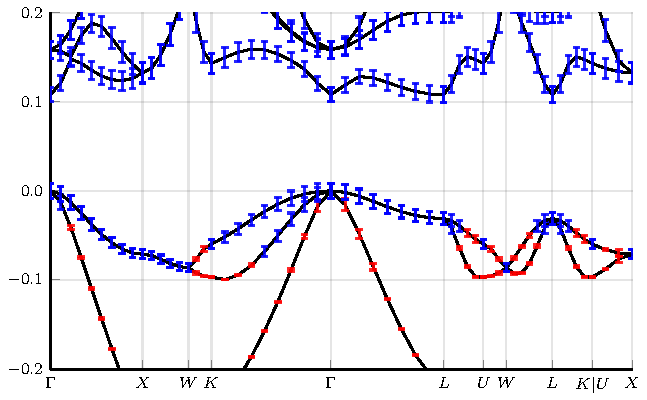
\includegraphics[width=0.7\textwidth]{img/si_band_errors.pdf}
        \end{center}
        \vspace{0.5em}
        \item Let's have a brief look at last year's projects \ldots
    \end{itemize}
\end{frame}

\begin{frame}{Questions ?}
    \begin{center}
        \huge{Questions ?}
    \end{center}
\end{frame}
